\section{Quantum algorithms}

It's now to see some important quantum circuits that can be used in practice in order to obtain interesting results or behaviour inside a quantum computer. A lot of them will be not usefull per se, but are really important for the creation of larger and more powerful schemes.

\subsection{Quantum Fourier Transform}

The aim is to create an algorithm that bring the computational basis into the Fourier base, defined by the application of the Fourier transform on the vectors of the base itself. Therefore, we need first to recall the definition of discrete fourier transform which is given by.
\dfn{Discrete Fourier transform}
{
    Taken a vector $(x_1, x_2, \dots, x_N)\in \mathbb{C}^N$ it's Fourier transform is an application $\mathcal{U}: \mathbb{C}^N \to \mathbb{C}^N$ that actes in the following way
    \begin{align}
        &\mathcal{U}\vb{x} = \vb{y}, &y_k = \frac{1}{\sqrt{N}} \sum_{j=1}^N e^{i2\pi \frac{jk}{N}}x_j.
    \end{align} 
}
\noindent
We know that such an application posses a lot of properties, in particular we know how the following realtions are true
\begin{align}
    \label{eq:DiscrFourTrans}
    &\mathcal{U}^{-1} = \mathcal{U}^*, &\mathcal{U}^{-1} = \mathcal{U}^\dagger,
\end{align}
meanging that it's a particular unitary transformation, and so we imagine that a circuit can represent it.

We basically want to create an algorithm that allows us to take the computational basis and perform \eqref{eq:DiscrFourTrans} on it. In order to do that we will use a particular notation to describe the computational base of an $N$ qubit system, using the binary representation.
\dfn{Binary representation}
{
    Taken a system of $N$ qubit, where the computational base has the form $\{\ket{00\dots 0}, \ket{00\dots 1}, \dots\}$ we will write down the element s of the basis as $\{\ket{j}\}_{j=0}^{2^N-1}$ where the following relation is given
    \begin{align}
        &\ket{j} = \ket{j_1j_2\dots j_N}, &j = \sum_{i=1}^N j_i 2^{N-i}.
    \end{align}
    basically $j$ is the number described by the system state in binary base.
}
\noindent
Using this notation it's really easy to write down the Fourier transform of the base having that
\begin{equation}
    \label{eq:QFT}
    \mathcal{U}\ket{j} = \frac{1}{2^{N/2}} \sum_{k=0}^{2^N-1} e^{i2\pi \frac{jk}{2^N}} \ket{k},
\end{equation}
having that the base is brought into another more complicated one. In fact, we can see how the states transform accordingly to the FT if the transformation is applied to the base. For example take a general state $\ket{\psi}$ we can see how
\begin{align}
    &\ket{\psi} = \sum_j x_j \ket{j}, &\mathcal{U}\ket{\psi} = \frac{1}{2^{N/2}} \sum_k\sum_j x_j e^{i2\pi \frac{jk}{2^N}} \ket{k} = \sum_k y_k\ket{k},
\end{align}
basically the coefficients defining the state in vector representation gets Fourier transformed. Still, this form of the Fourier tranform leaves not too much room for the creation of an algorithm that allow us to perform it in practice, so we need first to work a little on it and see how the following result holds.
\thm{Quantum Fourier Tranform}
{
    The Fourier transformation of the states in the computational basis can be rewritten as a sum of tensor product given by the following form using the binary representation for the base
    \begin{equation}
        \mathcal{U}\ket{j} = \frac{1}{2^{N/2}}\bigotimes_{l=1}^N\left[ \ket{0}_l + e^{i2\pi \mathbb{0}_j(N-l)}\ket{1}_l \right].
    \end{equation}
    Where the notation $\mathbb{0}_j(l)$ is defined as the following decimal number
    \begin{align}
        \label{eq:decimalForm}
        &\mathbb{0}_j(l) = \sum_{i=l+1}^N j_i2^{l - i}.
    \end{align}
}
\pf{Proof}
{
    We can start to work around the expression of \eqref{eq:QFT} by seing how we can rewrite $k/2^{N}$ in a more usefull form as
    \begin{equation}
        \frac{k}{2^N} = \sum_{l=1}^N k_l 2^{-l}.
    \end{equation}
    We can then substitute it and see how, recalling that $\ket{k} = \ket{k_1}\otimes\ket{k_2}\dots\otimes\ket{k_N}$, the following is true
    \begin{equation}
        \mathcal{U}\ket{j} = \frac{1}{2^{N/2}} \sum_{k=0}^{2^N-1} e^{i2\pi j\sum_{l=1}^N k_l 2^{-l}} \ket{k} = \frac{1}{2^{N/2}}\sum_{k=0}^{2^N - 1}\bigotimes_{l=1}^N e^{i2\pi jk_l 2^{-l}}\ket{k_l}.
    \end{equation}
    Now, the order of the operation can be inverted by taking some care anbd see how the expression become
    \begin{equation}
        \mathcal{U}\ket{j} = \frac{1}{2^{N/2}}\bigotimes_{l=1}^N \sum_{k_l = 0, 1}e^{i2\pi jk_l 2^{-l}}\ket{k_l} = \frac{1}{2^{N/2}}\bigotimes_{l=1}^N\left[ \ket{0}_l + e^{i2\pi j2^{-l}}\ket{1}_l \right].
    \end{equation}
    Now, we can see how the exponent can be simplified. In fact, if you use the definition of $j$ we can see how
    \begin{equation}
        j2^{-l} = \sum_i j_i 2^{N - i - l} = \sum_{i \le N-l} j_i 2^{N - i - l} + \sum_{i = N-l+1}^N j_i 2^{N - i - l} = \text{integer} + \mathbb{0}_j(N-l).
    \end{equation}
    Obviously the integer part gives no contribution to the phase since multiply $2\pi$ at the exponent, so only the $\mathbb{0}_j(N-l)$ can be written obtaining the final result.
}

\begin{figure}[t]
    \centering
    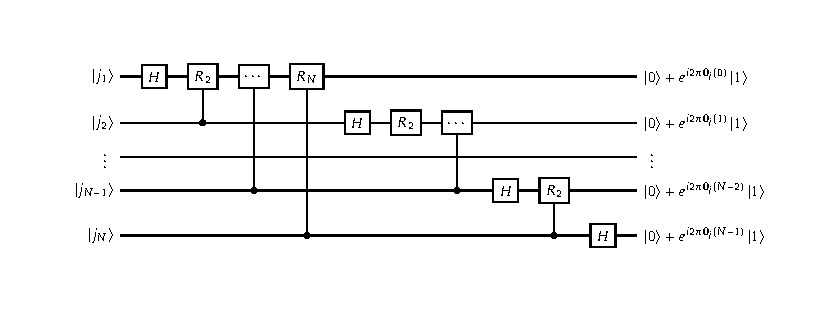
\includegraphics[width=0.9\textwidth]{Immagini/QFT.pdf}
    \caption
    {
        Circuits able to perform the quantum fourier tranform of the computational basis. It's important to notice how this algorithm is in reality not totally complete since the phases of the final states are inverted, so a series of swap gates needs to be inserted at the end to get the right form.
    }
    \label{fig:QFT}
\end{figure}
Now, this form of the QFT is much more usefull on an algorithmic point of view since it's now easy per us to see the operations that needs to be done on the single qubits. In particular, to reproduce the result we will need two types of gates that are also easy to understand that are
\begin{align}
    &H = \frac{1}{\sqrt{2}}\begin{pmatrix}
        1 & 1\\
        1 & -1
    \end{pmatrix},
    &R_k = \begin{pmatrix}
        1 & 0\\
        1 & e^{1\frac{2\pi}{2^k}}
    \end{pmatrix},
\end{align}
basically the Hadamart and phase gates. The final form of the circuit is described in \figref{fig:QFT}, where is possible to see how we can evaluate the QFT by the cimple use of controlled phase gates and swaps ones at teh end of the proces. This particular circuit is interesting since shows how quantum computers are able to perform fuorier transforms easily respect to classical algorithm. In fact, the number of gates required to perform such an operation scales as $\mathcal{O}(n^2)$ while the number of logic gates needed to perform the computation of a fast fourier transform inside a classical computer scales as $\mathcal{O}(n2^n)$. Quantum algorithm beats the classical one by an exponential factor. Nevertheless, the quantum algorithm has the big problem that the information are present in the phase of the states, and we are not able to evaluate them, basically meaning that the algorithm alone is useless. Still, we will see that QFT will still be used inside larger algorithm giving a lot of benefits.

\subsection{Phase evaluation}

The evaluation of phases inside quantum systems is always a troublesome problem, to the point that most of the time is thought as an impossible task. Nevertheless, is possible to see how the QFT algorithm is able to give us the possibility of experimentally evaluate a certain type of phase inside the system.

Let's imagine having a unitary operator $\mathcal{U}$ and wanting to evaluate the eigenvalues $\lambda_n$. We know from linear algebra that $\mathcal{U}\mathcal{U}^\dagger = \mathbb{1}$, so that from linear algebra we have the following information on the eigenvalues
\begin{align}
    &\lambda_n\lambda_n^* = \abs{\lambda_n}^2 = 1.
\end{align}
This relation tells us that the eigenvalues of such opeartors needs to be some kind of complex phases writable as
\begin{align}
    &\lambda_n = e^{2\pi i \phi_n}, &\phi_n \in [0, 1[.
\end{align}
Normally we would think that evaluating $\phi_n$ would be impossible since phases cannot be observed axperimentally. Still, we will show how using the eigenstate of the phases $\ket{u_n}$ and a simple operator $\mathcal{U}^{2^j}$ defined as follows
\begin{equation}
    \mathcal{U}^{2^j}: \ket{u_n} \longmapsto e^{2\pi i \phi_n 2^j} \ket{u_n},
\end{equation}
we are able to approximate its value with a wanted precision. In particular, we are aiming to approximate $\phi_n$ using a decimal form like the one in \eqref{eq:decimalForm}, so that we want to find $(b_n^1, b_n^2, \dots, b_n^t)$ so that 
\begin{equation}
    b_n = \frac{b_n^1}{2} + \frac{b_n^2}{4} + \dots + \frac{b_n^t}{2^t},
\end{equation}
is the decimal number $b < \phi_n$ closer to it as possible. Therefore, we are going to demonstrate that the algorithm showed in \figref{fig:Phase} is able to do exactly that, find out the values of $b_n^i$ approximating the phase up to a wanted accuracy.

\begin{figure}[t]
    \centering
    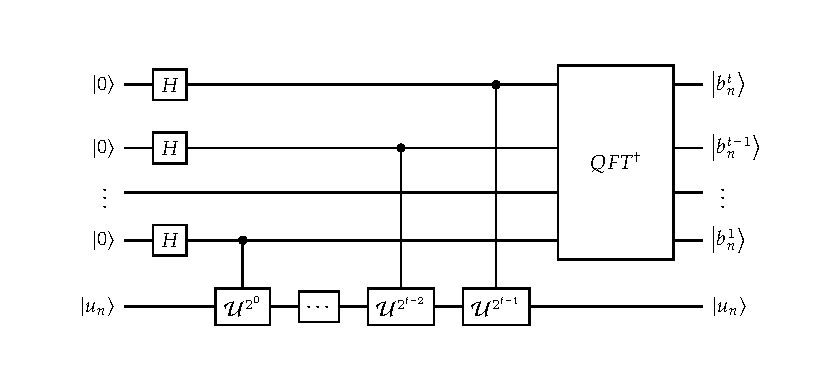
\includegraphics[width=0.8\textwidth]{Immagini/Phase.pdf}
    \caption
    {
        Quantum circuit for the approximation of the eigenvalues of a unitary operator up to a wanted accuracy based on the number of qubit used for the decimal approximation of the phase itself.
    }
    \label{fig:Phase}
\end{figure}

\thm{Phase evaluation}
{
    Taken a unitary operator $\mathcal{U}$ with eigenvalues defined by the phases $\phi_n$, the circuit \figref{fig:Phase} is able to give as output its decimal approximation $b_n$ with a wanted accuracy $\alpha > 0$, and precision $\epsilon > 0$ if the number of qubit used for the operation is
    \begin{equation}
        \label{eq:PhaseEvaluation}
        t > \alpha + \ln\left( 2 + \frac{1}{2\epsilon} \right).
    \end{equation}
}
\pf{Proof}
{
    First we need to look at what the circuit does effectivelly to the states, and it's easy to see that by looking at the case where $t = 1$ and see how the first part of the circuit works as follows
    \begin{equation}
        \left(C\mathcal{U}^{2^0}\right)\left(H\otimes\mathbb{1}\right)\ket{0}\otimes\ket{u_n} = C\mathcal{U}^{2^0}\left( \frac{\ket{0} + \ket{1}}{\sqrt{2}} \right)\otimes\ket{u_n} = \left( \frac{\ket{0} + e^{2\pi i\phi_n}\ket{1}}{\sqrt{2}} \right)\otimes\ket{u_n}.
    \end{equation}
    Which can be easily generalized to all the applications on the genearal $t$-dimensional circuit having a final form of the state given by
    \begin{equation}
        \ket{\psi_f} = \left[\bigotimes_{j = 0}^{t-1}\left( \frac{\ket{0} + e^{2\pi i\phi_n2^j}\ket{1}}{\sqrt{2}} \right)\right]\otimes\ket{u_n}
    \end{equation}
    Now, we know how every real number can be written as a converging series of rational numbers such as \eqref{eq:decimalForm} so that we are going to work with
    \begin{equation}
        \label{eq:rationalApproxPhase}
        \phi_n = \frac{\phi_n^1}{2} + \frac{\phi_n^2}{4} + \dots = \sum_{i=1}^\infty \frac{\phi_i}{2^i} \approx \sum_{i=1}^t \frac{\phi_i}{2^i}.
    \end{equation} 
    Meaning that can be approximated using the decimal representation described before, having that the phases can be rewritten using the following form
    \begin{equation}
        \exp\left( 2\pi i \phi_n 2^j \right) = \exp\left( 2\pi i\left\{ \left[ \phi_n^1 2^{j-1} + \dots \right] + \left[ \phi_n^{j+1}2^{-1} + \dots \right] \right\} \right) = \exp\left( 2\pi i \mathbb{0}_\phi(j) \right),
    \end{equation}
    where the first part was an integer giving no contribution. In this way one can understand that in the first part of the $\ket{\psi_f}$ state we end up having the QFT of the initial states, allowing us to write it in binary representation as
    \begin{equation}
        \ket{\psi_f} \approx \left( \frac{1}{2^{t/2}}\sum_{k=0}^{2^t-1}e^{2\pi i\phi_nk}\ket{k} \right)\otimes\ket{u_n}.
    \end{equation}
    In this way we can go and apply the inverse of the QFT and using the binary representation of the base to see what happens exactly in the transformation
    \begin{equation}
        QFT^\dagger \ket{\psi_f} = \frac{1}{2^t}\sum_{k=0}^{2^t-1} e^{2\pi i\phi_nk}\sum_{l=0}^{2^t-1} e^{-2\pi ikl/2^t}\ket{l} = \sum_l\left( \sum_{k=0}^{2^t-1}\frac{1}{2^t}e^{2\pi i (\phi_n - l/2^t)k} \right)\ket{l} = \sum_l c_l\ket{l}.
    \end{equation}
    The state becomes a superposition of states in the binary computational base of the $t$ qubits, and we know also the form of the coefficients. In fact, we can easily see how $c_l$ are composed by a geometric series giving rise to the following result
    \begin{equation}
        \label{eq:CoeffPhase}
        c_l = \frac{1}{2^t} \sum_{k=0}^{2^t-1} \left( e^{2\pi i (\phi_n - l/2^t)} \right)^k = \frac{1}{2^t}\frac{1 - e^{2\pi i (\phi_n - l/2^t)2^t}}{1 - e^{2\pi i (\phi_n - l/2^t)}}.  
    \end{equation}
    It's interesting to see how this result was obtained by truncating the real form of $\phi_n$ to a certain decimal order, but the procedure is general and works also in the case where the total series is retained. 
    
    Therefore, in \eqref{eq:CoeffPhase} the value of $\phi_n$ can be a rational or irrational number, and we can see what happens to $c_l$ in the two cases. In the case $\phi_n$ is rational we have that the approximation \eqref{eq:rationalApproxPhase} is exact, and we can write how
    \begin{equation}
        (\phi_n - l/2^t)2^t = \sum_{i=1}^t \phi_n^i 2^{t-i} -l = int.
    \end{equation}
    This means that the phase on the numerator of $c_l$ is a multiple of $2\pi$ and therefore $c_l = 0$ for every value of $l$ exept for $l=\phi_n 2^t$, where
    \begin{equation}
        c_{\phi_n2^t} = \frac{1}{2^t} \sum_{k=0}^{2^t-1} \left( e^{2\pi i (\phi_n - \phi_n)} \right)^k = \frac{2^t}{2^t} = 1.
    \end{equation}
    This means that $c_l = \delta_{l\phi_n2^t}$ which basically becomes a condition on the values of the single qubit that will take the following forms
    \begin{equation}
        \sum_{l=0}^{2^t-1} \delta_{l\phi_n2^t}\ket{l} = \ket{\phi_n2^t} = \ket{\phi_n^1}\otimes\ket{\phi_n^2}\otimes\dots\otimes\ket{\phi_n^t}, 
    \end{equation}
    where the binary representation was used to write down the single qubits. Now, we can simply evaluate all the $t$ qubits and have our approximation of the phase $\phi_n$ that is exact in this case, having that $b_n = \phi_n$.

    In the case $\phi_n$ is irrational, the truncation in the series generate an error having also that $(\phi_n - l/2^t)2^t$ is not an integer anymore and $c_l$ can be different from $0$ for other $l$ values. In this case we are going to approximate the value of $\phi_n$ using the values of $b_n$ that we obtain from the evaluation, and we want to know the error we are generating from such an approximation along with the accuracy of the result. Therefore, we select an error value $\omega$ and compute the probability of performing the measure 
    \begin{equation}
        \tilde{P} = P(\overline{l} \in [-\omega-1, \omega+1]),
    \end{equation}
    where $\overline{l} = l - \phi_n$ so that $\overline{l} = 0$ correspond to the real $\phi_n$. This evaluation can be performed using as $\omega$ the value $2^{t - \alpha} - 1$, where $\alpha$ is called accuracy, obtaining the result of
    \begin{equation}
        1 - \tilde{P} \le \frac{1}{2(2^{t-\alpha} - 2)}.
    \end{equation}
    Which identify the probability of not obtaining the wanted result, that we are going to set below a certain precision $\epsilon$ having $1 - \tilde{P}<\epsilon$ so that the following relations is found
    \begin{equation}
        t > \alpha + \ln\left( 2 + \frac{1}{2\epsilon} \right).
    \end{equation}
}
\noindent
Therefore, this algorithm is able to give us a really greate approximation for the phase that increase in accuracy as we scale up the number of qubit used in order to perform the operation. Also, it's possible to see how we from the inequality we can actually controll also the accuracy and precision of the prediction by setting them prior and then choose $t$ in order to satisfy \eqref{eq:PhaseEvaluation}.

\subsection{Grover algorithm}

Search algorithm are one of the most important type of algorithm that exist, since the aim is to find out specific elements inside a set that satisfy some requirements defined by ceratin function $f(x)$. Normally this kind of algorithms are really expensive scaling up real quick with both dimensions of the set and complexity of the function to use, but inside a quantum computer we can try to create a really efficient version of them.

Let's imagine to work with $n$ qubits, so that the computational base is composed by $N = 2^n$ elements that compose our set $\mathcal{N}$ in which only $1 \le M \le N$ elements are solutions of $f(x)$. Where, being solutions means that the state $\ket{x}$\footnote{We are using the binary representation for the state of the computational basis.} that represent that element is so that
\begin{equation}
    f(x) = \begin{cases}
        1 & x \in \text{solution}\\
        0 & x \notin \text{solution}
    \end{cases},
\end{equation}
basically $f: \mathcal{S} \to \{0, 1\}$ is a boolean function that gives true if it's solution and false otherwise. Then, we are going to need two types of gates that will generate the building blocks of our algorithm.
\thm{Oracle gate}
{
    The circuit shown in \figref{fig:oracle} is called oracle and is able to perform an inversion of the states that are not solution by using an ausiliary qubit in the $\ket{1}$ state.
    \begin{equation}
        \mathcal{O}\ket{x} = (-1)^{f(x)}\ket{x},
    \end{equation}
    so that if $\ket{x}$ is solution a $-1$ pops up, and remains equal otherwise.
}
\begin{figure}[t]
    \centering
    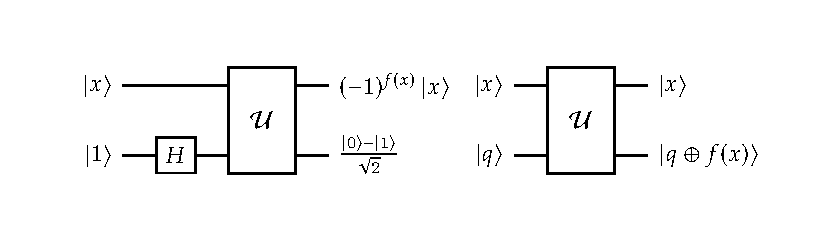
\includegraphics[width=0.8\textwidth]{Immagini/Oracle.pdf}
    \caption
    {
        Quantum circuit for the oracle gate used inside the algorithm to perform an inversion of the state about the components that are not solution to the function that we are interested in.
    }
    \label{fig:oracle}
\end{figure}
\pf{Proof}
{
    We can simply go over the different steps of the circuit to see how the following happens to the state
    \begin{equation}
        \mathcal{U}\left( \mathbb{1}\otimes H \right)\ket{x}\otimes\ket{1} = \mathcal{U}\ket{x}\otimes\left( \frac{\ket{0} - \ket{1}}{\sqrt{2}} \right) = \ket{x}\otimes\frac{1}{\sqrt{2}}\begin{cases}
            \ket{0} - \ket{1} & x \in \mathcal{S},\\
            \ket{1} - \ket{0} & x \in \mathcal{E}
        \end{cases}.
    \end{equation}
    Where $\mathcal{S}$ and $\mathcal{E}$ are the subset of $\mathcal{N}$ that contains the states that are solutions and not, respectivelly. Now, we can see how the difference between the two is simply a minus sign that we can imagine factorizing so that $\ket{x}$ takes it changing its phase as wanted.
}
\noindent
The next step is to define another type of gate that will be needed to perform another, more complex, type of reflection about the average state. Such gate is actually defined through also the use of a \textbf{conditional phase operator} defined as
\begin{equation}
    \mathcal{U}_x = 2\ketbra{x} - \mathbb{1},
\end{equation}
which has the effect of changing the phase to all state in the base that are not $\ket{x}$, and it's really easy to see since
\begin{align}
    &\mathcal{U}_x\ket{k} = \begin{cases}
        \ket{k} & k = x,\\
        -\ket{k} & k \neq x
    \end{cases}.
\end{align}
Using this idea we can define the wanted inversion operator in this particular way.
\thm{Inversion about the average}
{
    We can define the inversion about the average operator inside the space $\mathcal{N}$ as $\tilde{\mathcal{U}} = H^{\otimes n}\mathcal{U}_0 H^{\otimes n}$ and see how it's effect on a general state is
    \begin{align}
        &\ket{\phi} = \sum_{k\in\mathcal{N}}\alpha_k\ket{k}, &\tilde{\mathcal{U}}\ket{\phi} = \sum_{k\in\mathcal{N}}\left( 2\mean{\alpha} - \alpha_k \right) \ket{k}.
    \end{align}
    Which defines an inversion about the average state $\mean{\alpha}$.
}
\pf{Proof}
{
    We can first have a look at the form of the operator itself, which can be rewritten in a compact way as follows
    \begin{align}
        &\tilde{\mathcal{U}} = 2H^{\otimes n}\ketbra{0}H^{\otimes n} -\mathbb{1} = 2\ketbra{\psi} - \mathbb{1}, &\ket{\psi} = \frac{1}{\sqrt{N}}\sum_{k\in \mathcal{N}} \ket{k}.
    \end{align}
    Then, we can apply it to a general state to see how we retain the wanted result. In particular, we are going to write that
    \begin{align}
        &\tilde{\mathcal{U}}\sum_{k\in\mathcal{N}}\alpha_k\ket{k} = 2\sum_{k\in\mathcal{N}}\alpha_k\braket{\psi}{k}\ket{\psi} - \sum_{k\in\mathcal{N}}\alpha_k\ket{k} = 2\sum_{k\in\mathcal{N}}\sum_{l\in\mathcal{N}}\sum_{x\in\mathcal{N}}\frac{\alpha_k}{N} \braket{l}{k}\ket{x} - \sum_{k\in\mathcal{N}}\alpha_k\ket{k},
    \end{align}
    where we can use the fact that $\braket{l}{k} = \delta_{lk}$ to eliminate a summation and then see how $\sum_{k\in\mathcal{N}}\alpha_k/N = \mean{\alpha}$ so that the final result is obtained as
    \begin{equation}
        \tilde{\mathcal{U}}\sum_{k\in\mathcal{N}}\alpha_k\ket{k} = 2\sum_{x\in\mathcal{N}}\mean{\alpha}\ket{x} - \sum_{k\in\mathcal{N}}\alpha_k\ket{k} = \sum_{k\in\mathcal{N}}\left( 2\mean{\alpha} - \alpha_k \right) \ket{k}.
    \end{equation}
}

These two gates are the building blocks that will allow us to perform the quantum search and the idea to that is to actually define an operator that will allow us to transform the state into a linear combination of the ones that are solutions to our function. This can be done easily, since the following result holds, giving us the final form for the quantum search algorithm.
\thm{Quantum search}
{
    A general state $H^{\otimes n}\ket{0}$ can be decomposed in two main parts inside $\mathcal{N}$ as
    \begin{equation}
        \ket{\psi} = H^{\otimes n}\ket{0} = \sin\frac{\theta}{2}\ket{\beta} + \cos\frac{\theta}{2}\ket{\alpha},
    \end{equation}
    where $\ket{\beta}$ is a linear combination of all the solutions of $f(x)$, while $\ket{\alpha}$ a combination of all the non-solutions. The \textbf{Groover opeartor} $\mathcal{G} = \tilde{\mathcal{U}}\mathcal{O}$ acts on this state by rotating the angle $\theta$ in the direction of $\ket{\beta}$, so that if applied $R$ times we get
    \begin{equation}
        \mathcal{G}^R\ket{\psi} = \sin\left( \frac{2R + 1}{2}\theta \right)\ket{\beta} + \cos\left( \frac{2R + 1}{2}\theta \right)\ket{\alpha}.
    \end{equation}
    Therefore, we can select the right number of $\mathcal{G}$ to perform in order to obtain the maximum likelihood to obtain as a result of the measurament the state $\ket{\beta}$ with the solutions of the function.
}
\begin{figure}[t]
    \centering
    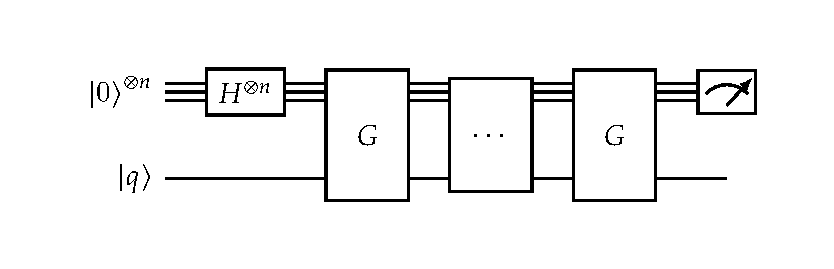
\includegraphics[width=0.7\textwidth]{Immagini/Groover.pdf}
    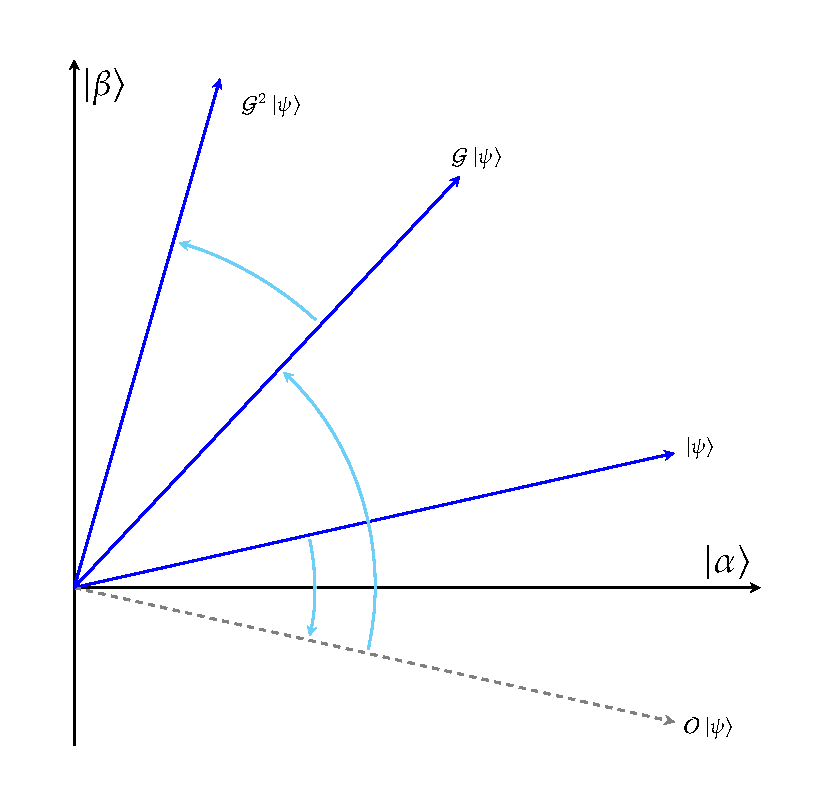
\includegraphics[width=0.25\textwidth]{Immagini/TrasfGrov.pdf}
    \caption
    {
        Graphical representation of the Groover's circuit, to the left, with transformations that happens to the state in the quantum search algorithm, to the right, in order to understand how the two reflection tranforms into a rotation.
    }
    \label{fig:Groover}
\end{figure}
\pf{Proof}
{
    We can start by looking at the general state $\ket{\psi}$ and see how can be rewritten as linear combination of solution and non-solution as follows
    \begin{equation}
        \ket{\psi} = \frac{1}{\sqrt{N}}\left( \sum_{k\in \mathcal{S}}\ket{k} + \sum_{k\in\mathcal{E}}\ket{k} \right) = \sqrt{\frac{M}{N}}\left( \frac{1}{\sqrt{M}}\sum_{k\in \mathcal{S}}\ket{k} \right) + \sqrt{\frac{N-M}{N}}\left( \frac{1}{\sqrt{N-M}}\sum_{k\in \mathcal{E}}\ket{k} \right),
    \end{equation}
    now we can see how $\sqrt{M/N}$ and $\sqrt{N-M/N}$ can be setted as the sine and cosine, while the superpositions that are mulitpling are exactly the linear combinations of all solutions and non-solutions respectivelly. Therefore, we effectivelly have that the following is true
    \begin{align}
        H^{\otimes n}\ket{0} = \sin\frac{\theta}{2}\ket{\beta} + \cos\frac{\theta}{2}\ket{\alpha},
    \end{align}
    then we shall see what the operator $\mathcal{G}$ does on it, and that can be done by looking at $\mathcal{O}$ and $\tilde{\mathcal{U}}$ separatelly. First, it's easy to understand how the oracle gate simply changes the sign of the $\ket{\beta}$ coefficient, meaning that using it simply performs a reflection of the state respec to the $\ket{\alpha}$ one. Then, the inversion by the average operator instead perform another inversion in this case that is respect to the state $\ket{\psi}$, so that two inversions apply one after giving a final rotation of the state as
    \begin{equation}
        \mathcal{G}\ket{\psi} = \sin\left( \frac{3}{2}\theta \right)\ket{\beta} + \cos\left( \frac{3}{2}\theta \right)\ket{\alpha},
    \end{equation}
    which is also depicted in \figref{fig:Groover}. Meaning that the rotation allowed for the state to become closer to the $\ket{\beta}$ state, and if we continue to perform it we will get as a state
    \begin{equation}
        \mathcal{G}^R\ket{\psi} = \sin\left( \frac{2R + 1}{2}\theta \right)\ket{\beta} + \cos\left( \frac{2R + 1}{2}\theta \right)\ket{\alpha}.
    \end{equation}
    In this way we can see how the probabilities of having as result $\ket{\beta}$ scales up since the angle gets closer to $\pi/2$, which gives $1$ as coefficient for that state. Still, it's possible to do too many rotations and ending up to go past the perfect value and increasing the coefficients for the $\ket{\alpha}$ state, still one can see how if $R$ is choosen as
    \begin{align}
        &R = \left[ \frac{\arccos\sqrt{M/N}}{\phi} \right], &\phi \le 4,
    \end{align}
    where $\left[ x \right]$ is the integer part function, we will have probabilities that looks like
    \begin{align}
        &P_\beta > 1/2, &P_\alpha < 1/2.
    \end{align}
    Basically, we can select $\phi$ to obtain the most optimized result possible, and already we know that by default the probabilities are in favor of the right result that we are serching for.
}
\noindent
Therefore, this algorithm allows us to search inside a set of states of dimensions $2^n$ the ones that satisfy the condition imposed by a wanted function $f$. Also, all of this is done by using a minimal number of operations that scales linearly with the number of qubit that we are using, beating in an increadible way the classical search algorithm that scales exponentially.

\subsection{Hamiltonian simulation}

On of the main goals that quantum computers scientists whant to achive is the possibility of simulate complex quantum systems efficiently thanks to the intrinsic quantum nature of QC themselfes. Basically the goal is to find a way to solve the SE inside a quantum computer finding out the time evolution operator of the system, which we recal in a time-independent $\mathcal{H}$ is
\begin{align}
    &\ket{\psi(t)} = \mathcal{U}(t)\ket{\psi_0}, &\mathcal{U}(t) = \exp\left( -i \frac{\mathcal{H}t}{\hbar} \right).
\end{align}
In order to do that we shall approximate the form of $\mathcal{U}(t)$ somehow using the qubit that we have avaliable, and the idea is the one of discretize it along with also $\ket{\psi}$. Basically, $\ket{\psi}$ will be thought as a function $\psi(\vb{x})$ where $\vb{x}\in\mathbb{R}^d$, and we are going to store only a set of values, of that function defined by the position on a lattice $\{x_j\}_j$, inside the qubit. Such discretization, then, nedds to be used also for the Hamiltionan, having an approximate form also for it, which define the evolution operator that we can then use to evolve the state.

To understand better how this is done we will assume that $\mathcal{H}$ is composed by a series of smaller components $\mathcal{H}_k$ containing only short range interactions, like
\begin{align}
    &\mathcal{H} = \sum_{k=1}^L \mathcal{H}_k = \sum_{\langle nm \rangle} Z_nZ_m +h\sum_l\left( Z_l + X_l \right).
\end{align}
This is an Ising Hamiltonian that has only on-site terms with longitudinal and trasversal field, and an interaction term that still applies only on nierest neighbours. Basically, we assume that $\mathcal{H}_k$ has interaction that at most account for a finite number of elements near a particular qubit. Inside these assumptions we can easily go and find out a way to approximate evolution operator by using a Taylor expansion as
\begin{equation}
    \label{eq:EasyApprox}
    \mathcal{U}(\Delta t) = \sum_{k=0}^\infty \frac{1}{k!}\left( -i\frac{\mathcal{H}\Delta t}{\hbar} \right)^k = \mathbb{1} - i\frac{\mathcal{H}\Delta t}{\hbar} + \mathcal{O}(\Delta t^2),
\end{equation}
where $\Delta t$ is the time discretization, assumed to be small. Also, from this poin on we will assume $\hbar = 1$ for simplicity of notation. We can see how the sum can be truncated to obtain an approximation of $\mathcal{U}$ that becomes better as the time discretization goes down, which is greate but not too greate. A better approach would be taking advantage of the decomposition of the Hamiltionian in pieces in order to rewrite the exponential as product of simpler operators that we know how to work with. Nevertheless, it's easy to see how also in the simple case we have looked at the $\mathcal{H}_k$ does not commute $\left[ \mathcal{H}_k, \mathcal{H}_m \right] \neq 0$, meaning that
\begin{equation}
    \exp\left( -it\sum_k\mathcal{H}_k \right) \neq \prod_{k}\exp(-it\mathcal{H}_k).
\end{equation}
This seems to set the sloppy \eqref{eq:EasyApprox} as the only possible way to approximate the operator, but it's not completely true. In fact, it's possible to demonstrate a result that saves the day.
\thm{Trotler decomposition}
{
    Taken two non commuting operators $A, B$ it's possible to decompose the exponential in the following way
    \begin{equation}
        \exp\left[ i\left( A + B \right)t \right] = \lim_{N\to\infty}\left( e^{i\frac{t}{N}A}e^{i\frac{t}{N}B} \right)^N.
    \end{equation}
}
\pf{Proof}
{
    We can use \eqref{eq:EasyApprox} to write down the following form
    \begin{equation}
        e^{i\frac{t}{N}A}e^{i\frac{t}{N}B} = \left[ \mathbb{1} - i\frac{\Delta t}{N}A + \mathcal{O}(1/N^2) \right]\left[ \mathbb{1} - i\frac{\Delta t}{N}B + \mathcal{O}(1/N^2) \right] = \mathbb{1} + i\frac{t}{N}\left( A + B \right) + \mathcal{O}(1/N^2),
    \end{equation}
    which elevated to the power of $N$ allow for the following result to show up
    \begin{equation}
        \left( e^{i\frac{t}{N}A}e^{i\frac{t}{N}B} \right)^N = \mathbb{1} + \sum_{K=1}^N \binom{N}{k}\frac{\left[ it\left( A + B \right) \right]^k}{N^k} + \mathcal{O}(1/N). 
    \end{equation}
    Here, is possible also to see how the binomial coefficents can be approximated in the following way
    \begin{equation}
        \binom{N}{k} \frac{1}{N^k} \sim \frac{1}{k!} + \mathcal{O}(1/N),
    \end{equation}
    having that the final form becomes exactly the sum of the Taylor expansion wanted in the limit of $N\to\infty$.
}
\noindent
Such a result allows for a better way to approximate the evolution operator by setting a ceratin discretization defined by $N$ and then perform several steps in the middle. This can be also done analitically to find out some important closed formulas in order to have a better computational approach, and the most used one is the \textbf{Baker Hausdorff formula}
\begin{equation}
    e^{i(A+B)\Delta t} = e^{iA\Delta t}e^{iB\Delta t} e^{-\frac{i}{2}[A, B]\Delta t^2} + \mathcal{O}(\Delta t^3).
\end{equation}
Which is a good improvment of the previous naive approximation.

Let's now imagine that we want to work in order to simulate a 1D particle inside a potential $V(x)$, we will have that the system is described as
\begin{align}
    &\mathcal{H} = \frac{\hat{p}^2}{2m} + V(\hat{x}), &x\in [-d, d].
\end{align}
In this situation we discretize the space to have a spacing $a = 2d/N$ and the points on the lattice that we are working with are described by the values
\begin{align}
    &x_j = aj, &j\in\left[ -N/2, N/2 \right].
\end{align}
In this way we will define the position basis as the set $\{x_j\}$ so that the following is true 
\begin{equation}
    V(\hat{x}) \ket{x_j} = V(x_j) \ket{x_j},
\end{equation}
having that they diagonalize the potential part of the Hamiltonian. Using this base also the state of the particle can be written as a linear combination of the type
\begin{equation}
    \ket{\psi} = \sum_{j = -N/2}^{N/2} \alpha_j \ket{x_j}.
\end{equation}
Therefore, this set allows for the discretization of both the state of the particle and a part of the Hamiltonian, to complete our needs we will need also to store the momentum part of the Hamiltonian, but it's not diagonal in such base. For this reason, the idea is to write $\hat{p}$ as the Fourier transform of the position operator $\mathcal{U}_{FT}\hat{x}\mathcal{U}_{FT}^\dagger$ since we know to perform the Fourier tranform of the state, meaning that we can effectivelly evaluate also $\hat{p}\ket{x_j}$ having all that we need.

\begin{figure}[t]
    \centering
    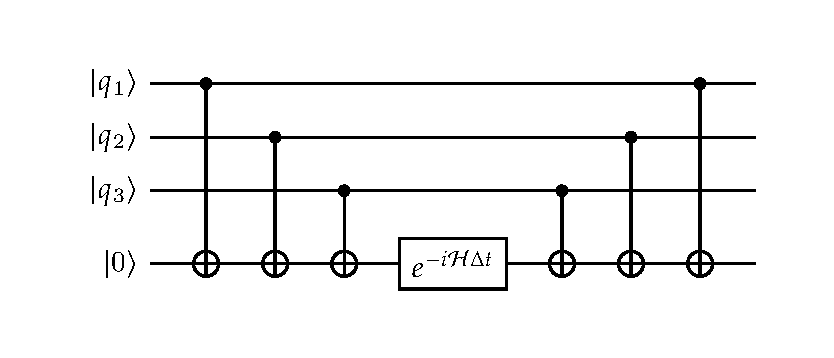
\includegraphics[width=0.8\textwidth]{Immagini/HSim.pdf}
    \caption{
        Quantum circuit used in order to simulate the simple system of the example, if the circuitis folled it's effectivelly possible to see how the final form is exactly the initial state plus the wanted phase and the ancilla qubit.
    }
    \label{fig:HSim}
\end{figure}

\ex{Simple case}
{
    The prof showed a really simple example of system simulation on a quantum computer, where the Hamiltonian is simply 
    \begin{equation}
        \mathcal{H} = Z_1\otimes Z_2\otimes Z_3,
    \end{equation}
    meaning that three qubit are studied and the base is so $\ket{q_1q_2q_3}$. We shall also remember that the effect of $Z$ is changing sign to the state if it's value is $1$ or not touching it otherwise. Knowing it allows us to find out how the Hamiltonian act on a general state having
    \begin{align}
        &\mathcal{H}\ket{q_1q_2q_3} = \delta_{q_1q_2q_3}\ket{q_1q_2q_3}, &\delta_{q_1q_2q_3} = \begin{cases}
            1 & \#1\text{ is even},\\
            -1 & \#1\text{ is odd}
        \end{cases}.
    \end{align}
    Using this we can implement a quantum circuit that simulates the evolution by adding the correct phase to a general state of the base every time is applied to it. The circuit we are talking about is represented in \figref{fig:HSim}, where one can see how the ancilla qubit will be $1$ befor the phase gate if an odd number of 1 are present in the initial state, and then will return to the initial state. Therefore, the final result is simply $e^{i\delta\Delta t}\ket{q_1q_2q_3}\otimes\ket{0}$, the state has effectivelly evolved as we wanted.
}